%                      Code_Saturne version 1.3
%                      ------------------------
%
%     This file is part of the Code_Saturne Kernel, element of the
%     Code_Saturne CFD tool.
% 
%     Copyright (C) 1998-2007 EDF S.A., France
%
%     contact: saturne-support@edf.fr
% 
%     The Code_Saturne Kernel is free software; you can redistribute it
%     and/or modify it under the terms of the GNU General Public License
%     as published by the Free Software Foundation; either version 2 of
%     the License, or (at your option) any later version.
% 
%     The Code_Saturne Kernel is distributed in the hope that it will be
%     useful, but WITHOUT ANY WARRANTY; without even the implied warranty
%     of MERCHANTABILITY or FITNESS FOR A PARTICULAR PURPOSE.  See the
%     GNU General Public License for more details.
% 
%     You should have received a copy of the GNU General Public License
%     along with the Code_Saturne Kernel; if not, write to the
%     Free Software Foundation, Inc.,
%     51 Franklin St, Fifth Floor,
%     Boston, MA  02110-1301  USA
%
%-----------------------------------------------------------------------
%

%%%%%%%%%%%%%%%%%%%%%%%%%%%%%%%%%%
%%%%%%%%%%%%%%%%%%%%%%%%%%%%%%%%%%
\section{Discr\'etisation} \label{Base_Viscfa_paragraphe2}
%%%%%%%%%%%%%%%%%%%%%%%%%%%%%%%%%%
%%%%%%%%%%%%%%%%%%%%%%%%%%%%%%%%%%
On rappelle dans la figure \ref{Base_Viscfa_fig_geom}, la d�finition des diff�rents
points g�om�triques utilis�s par la suite.

\begin{figure}[h]
\parbox{8cm}{%
\centerline{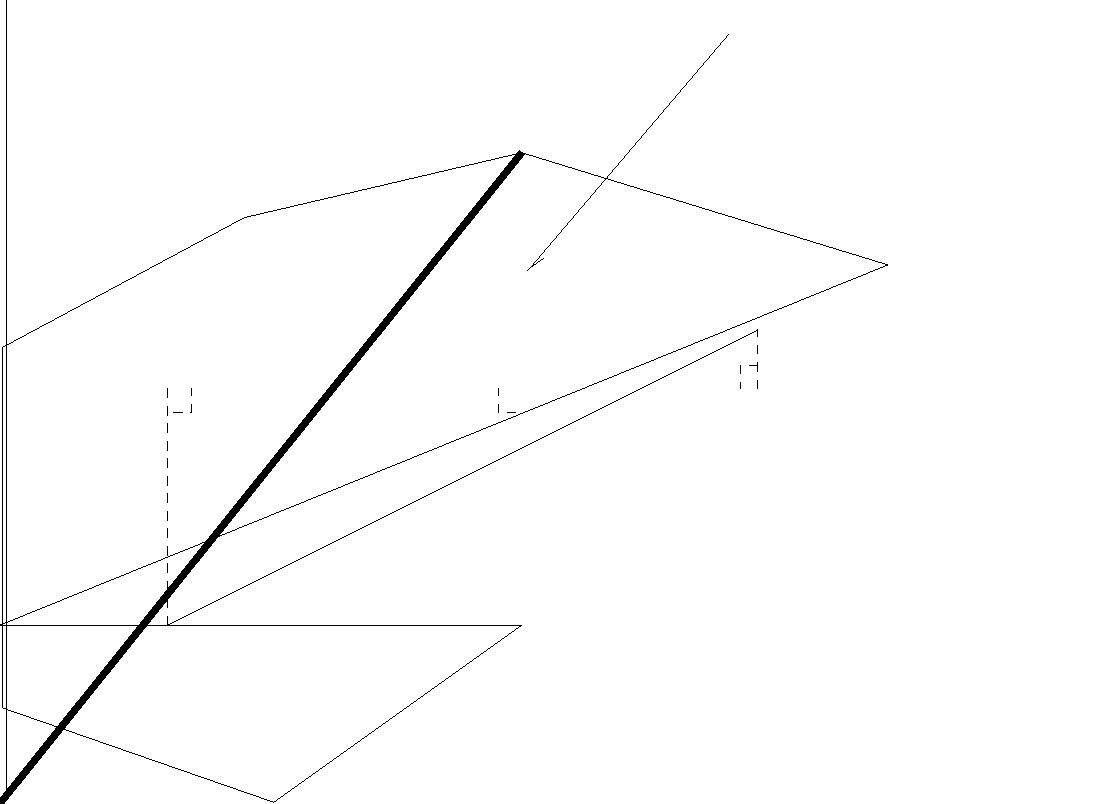
\includegraphics[height=4.5cm]{../Base/Viscfa/Images/facette.pdf}}}
\parbox{8cm}{%
\centerline{
\includegraphics[height=4.5cm]{../Base/Viscfa/Images/facebord.pdf}}}
\caption{\label{Base_Viscfa_fig_geom}D\'efinition des diff\'erentes entit\'es
g\'eom\'etriques pour les faces internes (gauche) et de bord (droite).}
\end{figure}

L'int�gration du terme de diffusion sur une cellule $\Omega_i$ est la suivante :
\begin{equation}
\int_{\Omega_i}\dive (\mu\,\grad(f))\,d\Omega= \sum\limits_{j \in
Vois(i)}\mu_{\,ij} \frac{f_{J'}-f_{I'}}{\overline{I'J'}}\,.\, S_{\,ij} + \sum\limits_{k \in
\gamma_b(i)}\mu_{\,b_{ik}} \frac{f_{\,b_{ik}}- f_{I'}}{\overline{I'F}}\,.\,S_{\,b_{ik}}
\end{equation}
Dans ce sous-programme, on calcule les termes de diffusion
$\displaystyle \mu_{\,ij}\frac{S_{\,ij}}{\overline{I'J'}}$ et $\displaystyle
\mu_{\,b_{ik}}\,.\,\frac{S_{\,b_{ik}}}{\overline{I'F}}$.\\

La valeur de la viscosit� sur la face interne $ij$, $\mu_{\,ij}$, est calcul�e :\\
\hspace*{1.cm} {\tiny$\bigstar$}  soit par moyenne arithm�tique :
\begin{equation}
\mu_{\,ij}=\alpha_{\,ij}\mu_{\,i}+(1-\alpha_{\,ij})\mu_{\,j}
\end{equation}
avec $\alpha_{\,ij} = 0.5$ car ce choix semble stabiliser, bien que cette
interpolation soit d'ordre 1 en espace en convergence.\\
\hspace*{1.cm} {\tiny$\bigstar$} soit par moyenne harmonique :
\begin{equation}\notag
\mu_{\,ij}=\frac{\mu_{\,i}\ \mu_{\,j}}{\alpha_{\,ij}\mu_{\,i}+(1-\alpha_{\,ij})\mu_{\,j}}
\end{equation} 
avec $\alpha_{\,ij}=\displaystyle \frac{\overline{FJ'}}{\overline{I'J'}}$.\\

La valeur de la viscosit� sur la face de bord $ik$, $\mu_{\,b_{ik}}$, est d�finie
ainsi :\\
\begin{equation}\notag
\mu_{\,b_{ik}}=\mu_I.
\end{equation}
\minititre{Remarque}
Lors de l'appel de \fort{viscfa} par le sous-programme \fort{resolp}, le terme
\`a consid\'erer est :
\begin{equation}\notag 
\dive (\,\Delta t^n \ \grad(\delta p)\,)
\end{equation}
soit :
\begin{equation}\notag 
\mu = \mu^n = \Delta t
\end{equation}  

